\documentclass[10pt,a4paper]{article}
\usepackage[utf8]{inputenc}
\usepackage[english]{babel}
\usepackage[T1]{fontenc}
\usepackage{amsmath}
\usepackage{amsfonts}
\usepackage{amssymb}
\usepackage{graphicx}
\usepackage{epstopdf}
\usepackage{float}
\usepackage[a4paper,left=3cm,right=3cm,top=2.5cm,bottom=1.5cm]{geometry}
\usepackage[hyperfootnotes=false,hidelinks]{hyperref}
\usepackage{gensymb}
\addtolength{\footnotesep}{3mm}
\usepackage[bottom]{footmisc}

\title{Magnetic Levitation}
\author{Kudlankográl GCHD}
\date{}

\makeatletter
\newcommand{\settitle}{\@maketitle}
\makeatother

\begin{document}


\settitle
\thispagestyle{empty}
\addtocounter{page}{-1}


\begin{figure}[H]
\centering
    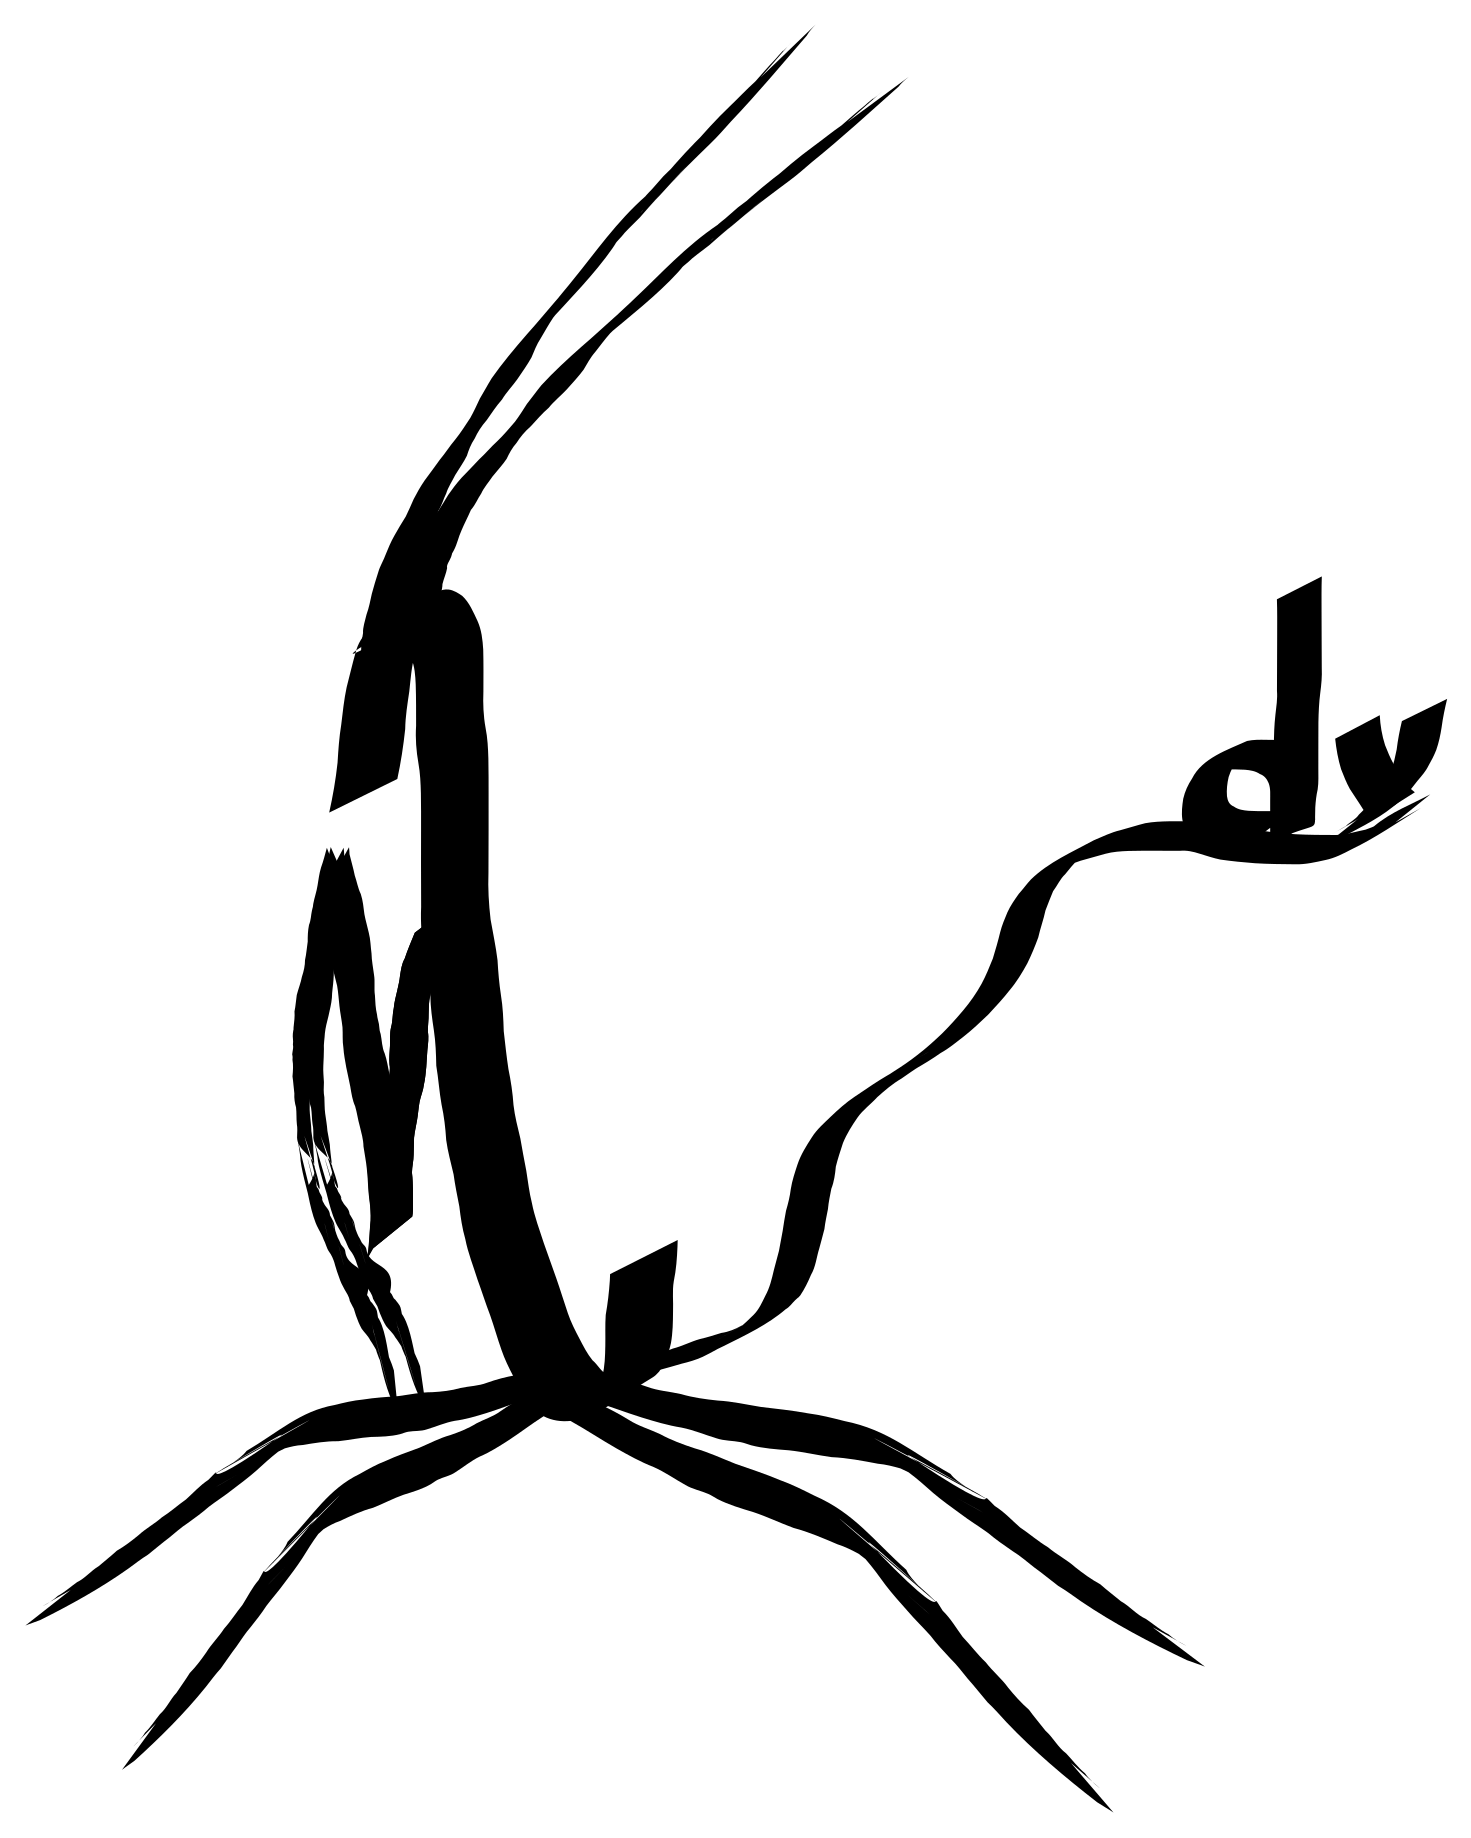
\includegraphics[width=0.95\textwidth]{kudlankogral.png}
\end{figure}

\paragraph{}
Name of the team: Kudlankográl GCHD
\paragraph{}
School: Gymnázium Christiana Dopplera
\paragraph{}
Address: Zborovská 621/45, Praha 5 - Malá Strana, 150 00

\clearpage
\newpage


\author{}
\maketitle

\section*{Abstract}
This paper focuses on describing the phenomenon of magnetic levitation of magnetic stirrer fleas in viscous fluids. Firstly, the equations involving the behavior of the stirrer flea are derived, and applied to  the specific condition of the flea levitating. The created model of the flea trajectory and height based on  stirring speed is then compared to measurements and observations made. Secondly, the phenomenon is investigated using system dynamics theory, and explores the role of fluid viscosity. Overall, the produced theoretical model and the empirical data are in good correlation.

\tableofcontents

\newpage

\section{Problem}
"Under certain circumstances, the “flea” of a magnetic stirrer can rise up and levitate stably in a viscous fluid during stirring. Investigate the origins of the dynamic stabilization of the “flea” and how it depends on the relevant parameters." (IYPT, 2019)

\section{Introduction}
A magnetic stirrer is a device, using magnetic forces to stir the contents of a beaker. To do so, a permanent magnet is placed inside the beaker (the “flea”), and two rotating magnets underneath the beaker cause it to spin rapidly, stirring the content of the beaker. Under certain circumstances, the flea will instead start to levitate inside the container.\par  This paper aims to give answers to why this phenomenon occurs, which magnet rotation speeds and fluid viscosities allow for this to happen, and how can this effect be modeled.\par A demonstrative video can be found alongside this work; it a slow-motion capture of the motion of a levitating flea. A distinctive vertical oscillation, as well as a horizontal rotation can be observed. A decomposition of flea motion into these two components will be used in our investigation, similarly to another research by Baldwin et al. (2018).

\section{Magnetic forces}
To understand the resulting phenomenon, it is necessary to first describe the magnetic forces between the magnets inside the stirrer and in the flea. The magnetic field has two effects on the flea (see image \ref{obr:michacka}): a vertical force and a horizontal rotational force. It can be assumed that the flea is centered in the axis of magnet rotation, and that it is always in a horizontal position. Two different models will be introduced, and compared to experimental data.

\begin{figure}[H]
  \centering
  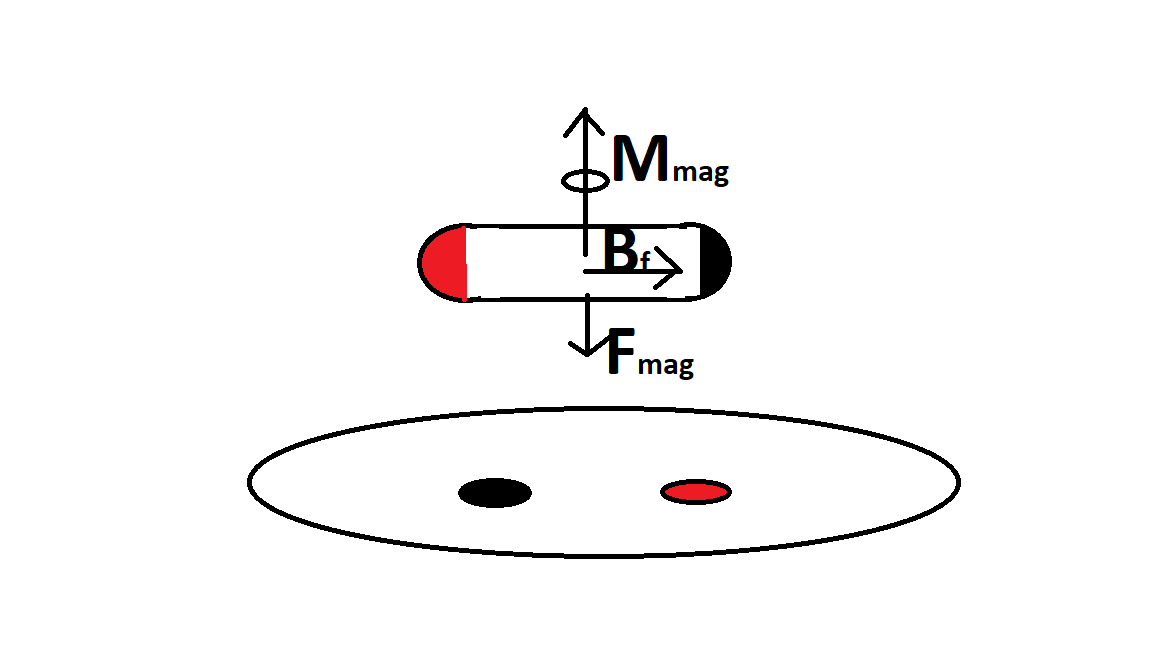
\includegraphics[width=0.5\textwidth]{michacka_sily_schema.png}
  \caption{A diagram of magnetic forces}
  \label{obr:michacka}
\end{figure}

\subsection{1 point dipole in flea and 1 in stirrer}
In this model, we approximate magnets in the flea and the stirrer as two magnetic dipoles of negligible size. The magnetic field from the stirrer magnet can then be described using the following equation (DSPS, 2017):
\begin{equation}
\vec{B} = \frac{\mu_{0}}{4 \pi} \left(\frac{\vec{m}_{st} \cdot \vec{r}}{r^5}\vec{r} - \frac{\vec{m}_{st}}{r^3}\right)
\label{indukce:dipol}
\end{equation}
$\vec{m_{st}} \cdot \vec{r}$ is equal to zero, given that the dipole moment is always perpendicular to the positional vector of the flea.
The equation, for a given height $h$, can therefore be reduced to:
\begin{equation}
\vec{B}_{f} = \frac{\mu_{0}}{4 \pi} \frac{\vec{m}_{st}}{h^3}
\label{indukce1dipol:blecha}
\end{equation}
The rotational moment of force is equal to the vector product of the dipole moment of the flea and the magnetic induction in the flea's location:
\begin{equation}
M_{mag} = |\vec{m}_f \times \vec{B}_f| = \frac{\mu_{0}}{4 \pi} \frac{\vec{m}_f\times \vec{m}_{st}}{h^3} = \frac{\mu_{0}}{4 \pi} \frac{|\vec{m}_f||\vec{m}_{st}|}{h^3}\sin(\theta_f - \theta_{st})
\label{moment1dipol}
\end{equation}
The vertical force is equal to the derivative of the scalar product of the dipole moment of the flea and the induction at the given point (DSPS, 2017):
\begin{equation}
F_{mag} = \frac{d}{dh} \vec{m}_f \cdot \vec{B}_f = \frac{\mu_{0}}{4 \pi} \frac{d}{dh} \frac{\vec{m}_f \cdot \vec{m}_{st}}{h^3} =  3 \frac{\mu_{0}}{4 \pi} \frac{|\vec{m}_f||\vec{m}_{st}|}{h^4}\cos(\theta_f - \theta_{st})
\label{sila1dipol}
\end{equation}
The resulting equation can be simplified by substituting all the constants present for a single constant.
\begin{equation}
 K_{mag} = \frac{\mu_{0}}{4 \pi}{|\vec{m}_f||\vec{m}_{st}|}
 \label{definiceKmag}
 \end{equation}
The equations can then be rewritten:
\begin{equation}
M_{mag} = \frac{K_{mag}}{h^3}\sin(\theta_f - \theta_{st})
\label{magmoment2}
\end{equation}
and
\begin{equation}
F_{mag} = 3\frac{K_{mag}}{h^4}\cos(\theta_f - \theta_{st})
\label{magsila2}
\end{equation}


\subsection{1 point dipole in flea and 2 in stirrer}
\begin{figure}[H]
  \centering
  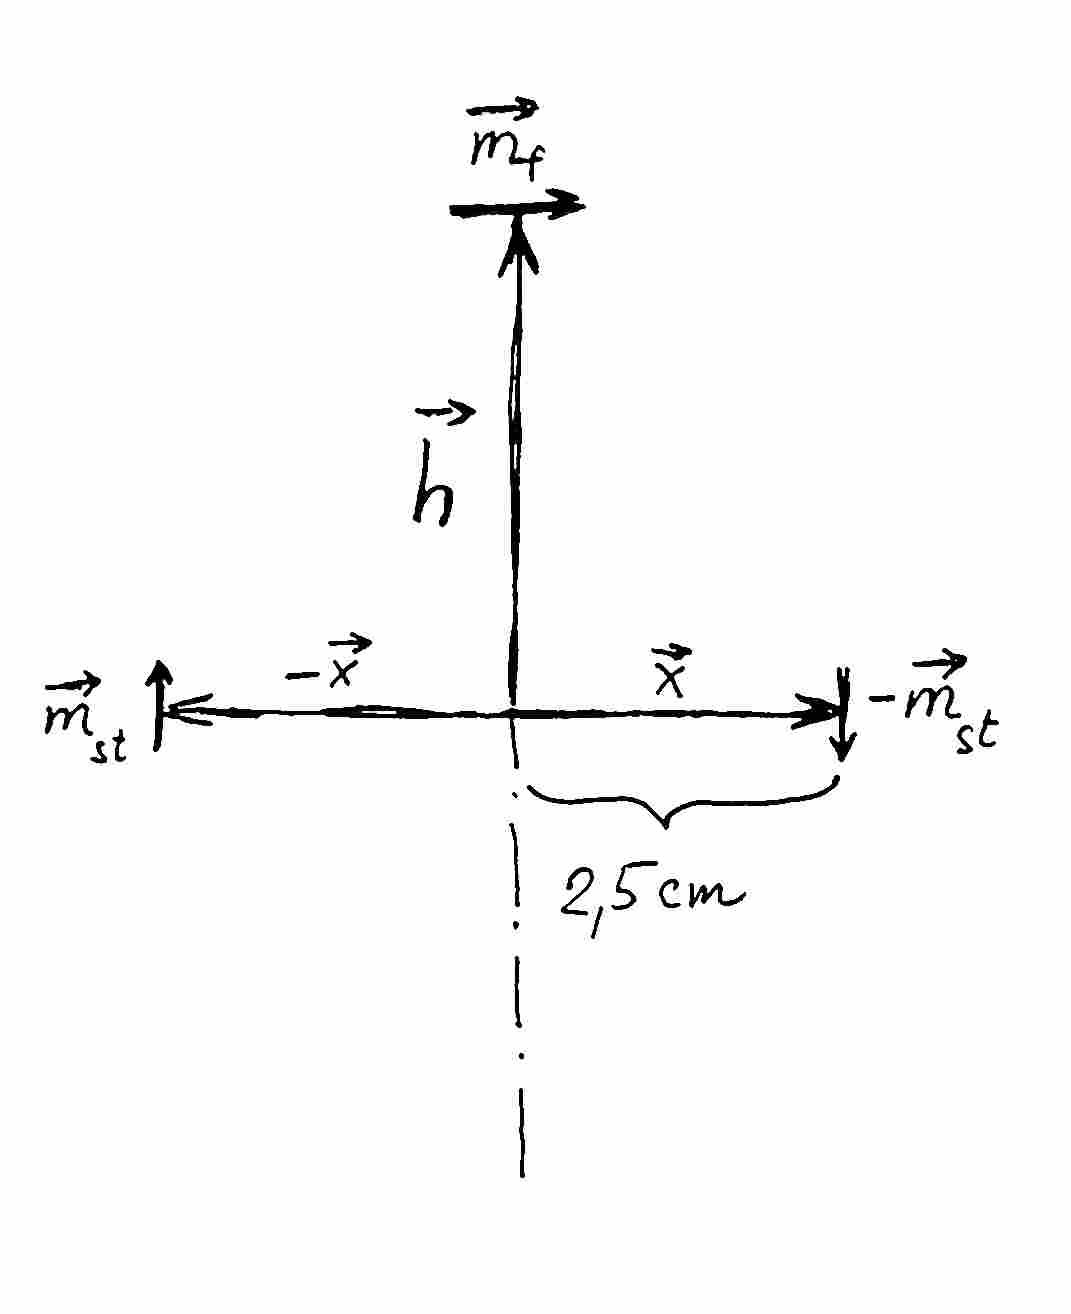
\includegraphics[width=0.5\textwidth]{Fig2a.jpg}
  \caption{A scheme of the 2nd model}
  \label{obr:2 dipoly}
\end{figure}

\begin{figure}[H]
  \centering
  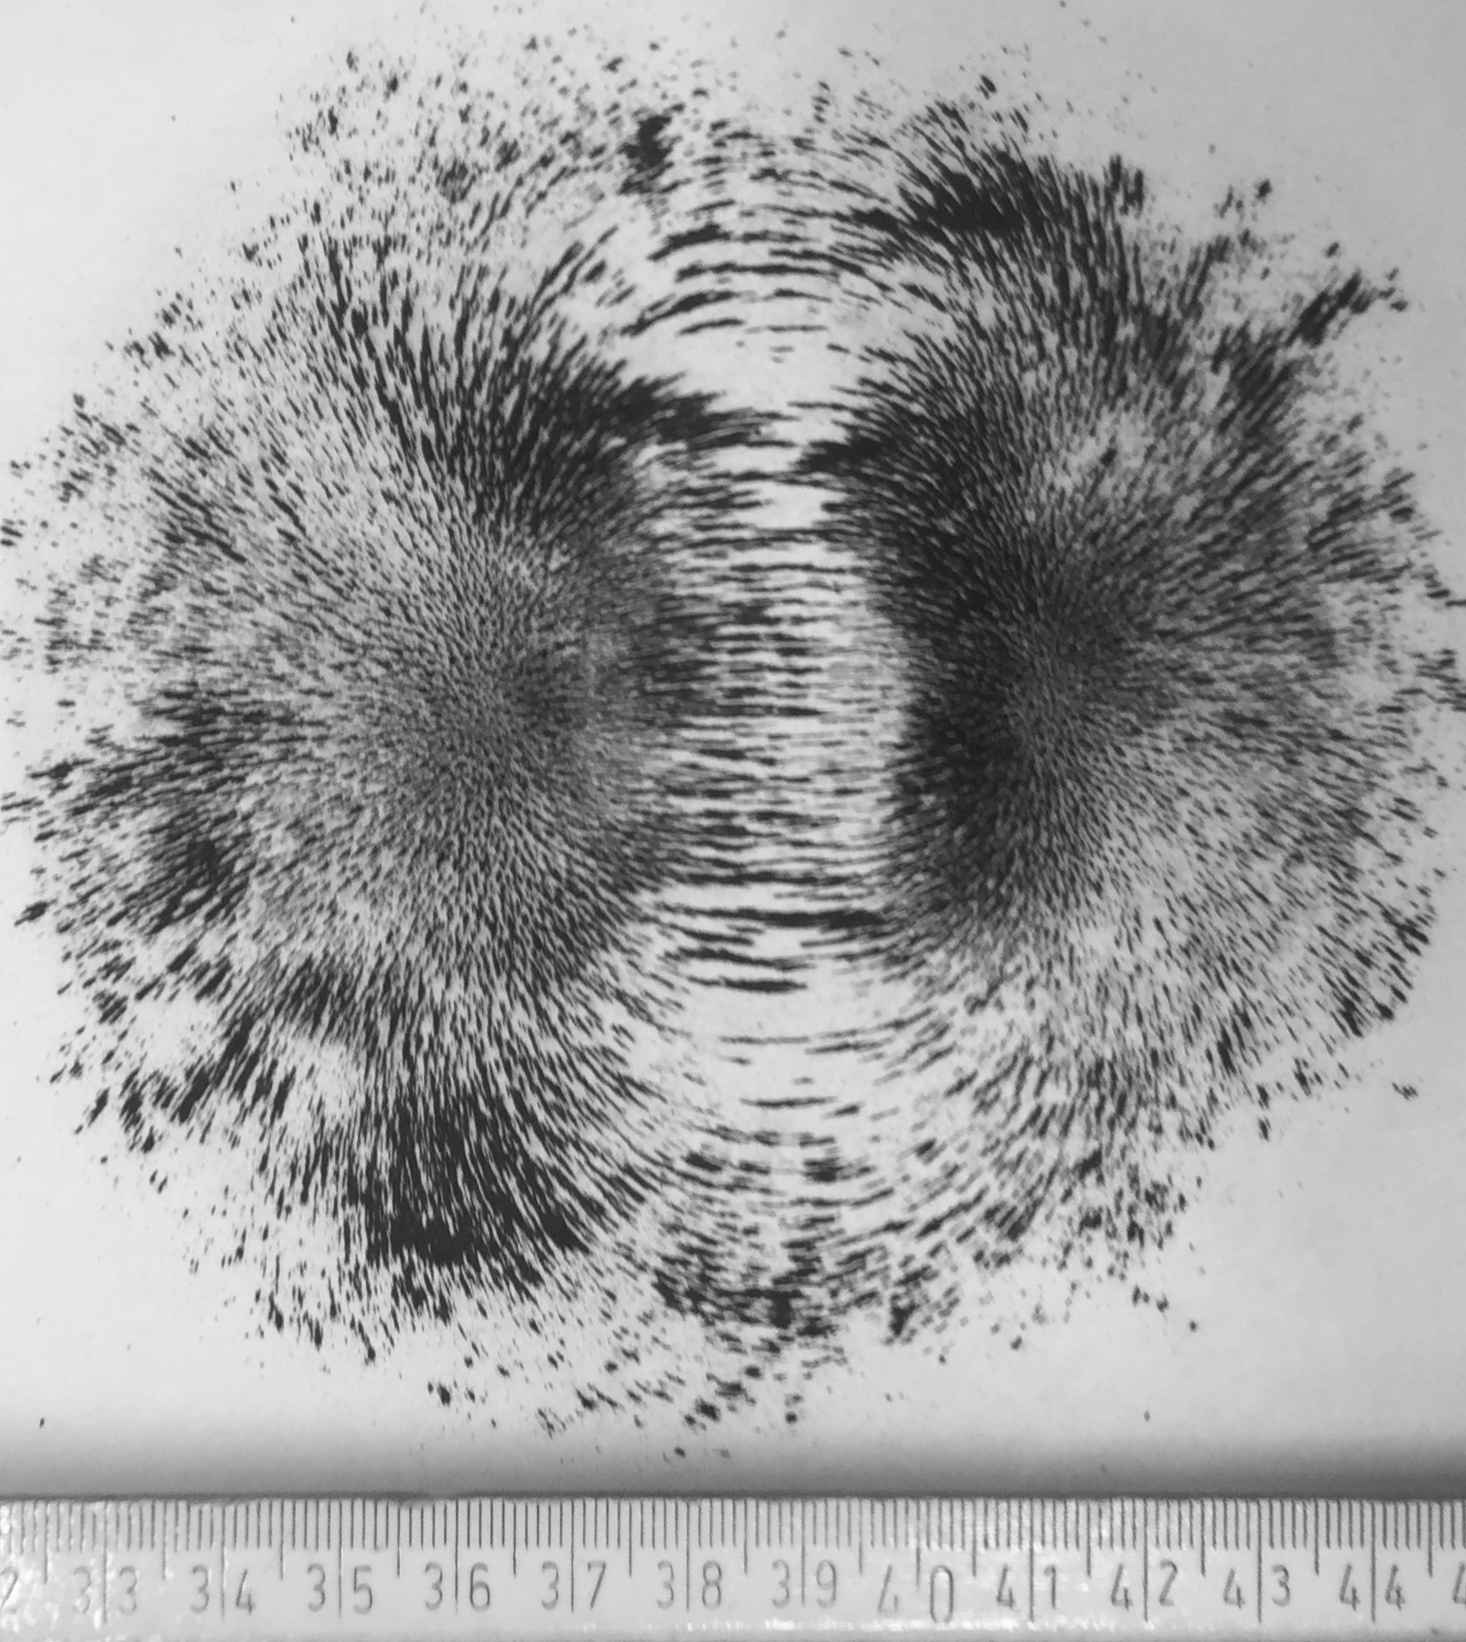
\includegraphics[width=0.5\textwidth]{Fig2b.jpg}
  \caption{A visualization of the magnetic field}
  \label{obr:piliny}
\end{figure}
This model is based on the fact, that there are two magnets present in the stirrer, oriented vertically – as visible in \ref{obr:2 dipoly} or in the visualization in \ref{obr:piliny} – and approximates them as two point dipoles. The distance of the magnets from the axis of rotation is $x$. The magnetic induction from one of the magnets is (DSPS, 2017):
\begin{equation}
\vec{B} = \frac{\mu_{0}}{4 \pi} \left(\frac{\vec{m}_{st} \cdot \vec{r}}{r^5}\vec{r} - \frac{\vec{m}_{st}}{r^3}\right)
\label{indukce2dipoly}
\end{equation}
The total induction in the point of the flea is equal to the superposition of inductions from both magnets. Because both of the magnets in the stirrer have equal, oppositely directed dipole moments, the $\frac{\vec{m_{st}}}{r^3}$ from both equations will cancel each other out, leaving:
\begin{equation}
\vec{B}_{f} = \frac{\mu_{0}}{4 \pi} \left( \frac{\vec{m}_{st} \cdot \left( \vec{h} + \vec{x} \right) }{|\left(\vec{h}+\vec{x}\right)|^5}  \left( \vec{h} + \vec{x} \right) - \frac{\vec{m}_{st} \cdot \left( \vec{h} - \vec{x} \right) }{|\left(\vec{h}-\vec{x}\right)|^5}  \left( \vec{h} - \vec{x} \right)\right)
\label{indukce2dipoly:blecha}
\end{equation}
Because the dipole moment is vertical, it is possible to further simplify the equation:
\begin{equation}
\vec{B}_{f} = \frac{\mu_{0}}{2 \pi} \frac{\vec{m}_{st} \cdot \vec{h}}{\left(\vec{h} +\vec{x}\right)^5} \vec{x} =  \frac{\mu_{0}}{2 \pi}  \frac{|\vec{m}_{st}||\vec{h}|  \vec{x}}{\sqrt{|\left(|\vec{h}|^2+|\vec{x}|^2\right)|^5}}
\label{indukce2dipoly:blecha2}
\end{equation}
Expressing the moment of force:
\begin{equation}
M_{mag} = |m_f \times \vec{B}_f| = |\frac{\mu_{0}}{2 \pi}  \frac{|\vec{m}_{st}|| \vec{h}|\vec{m}_f \times\vec{x}}{\sqrt{\left(|\vec{h}|^2+|\vec{x}|^2\right)^5}} |=  \frac{\mu_{0}}{2 \pi}  \frac{|\vec{m}_{st}|| \vec{h}||\vec{m}_f|| \vec{x}|}{\sqrt{\left(|\vec{h}|^2+|\vec{x}|^2\right)^5}} \sin(\theta_f - \theta_{st})
\label{moment2dipoly}
\end{equation}
And the vertical component of force:
\begin{equation}
F_{mag} = \frac{d \left(\vec{ m}_f \cdot \vec{B}_f \right)}{d h} = \frac{\mu_{0} }{2 \pi} \frac{d}{dh} \frac{|\vec{m}_{st} | |\vec{h}| \vec{x} \cdot \vec{m}_f}{\sqrt{\left(|\vec{h}|^2+|\vec{x}|^2\right)^5}}
\label{sila2dipoly}
\end{equation}
Which, after derivation, produces
\begin{equation}
 F_{mag} = \frac{\mu_{0} |\vec{m}_{st}||\vec{m}_f|| \vec{x}|}{2 \pi}  \left( \frac{1}{\sqrt{\left(|\vec{h}|^2+|\vec{x}|^2\right)^5}} - \frac{2.5|\vec{h}|}{\sqrt{\left(|\vec{h}|^2+|\vec{x}|^2\right)^7}} \right) \cos(\theta_f - \theta_{st})
 \label{sila2dipoly2}
 \end{equation}
The same constant (see equation \ref{definiceKmag}) can be used as in the previous model. The results are two equations:
\begin{equation}
 M_{mag} = 2 K_{mag}\frac{| \vec{h}|| \vec{x}|}{\sqrt{\left(|\vec{h}|^2+|\vec{x}|^2\right)^5}} \sin(\theta_f - \theta_{st})
 \label{2dipolymoment}
 \end{equation}
and
\begin{equation}
 F_{mag} = 2 K_{mag} |\vec{x}|\left( \frac{1}{\sqrt{\left(|\vec{h}|^2+|\vec{x}|^2\right)^5}} - \frac{2.5|\vec{h}|}{\sqrt{\left(|\vec{h}|^2+|\vec{x}|^2\right)^7}} \right) \cos(\theta_f - \theta_{st}) 
 \label{magsila2dipoly}
 \end{equation}

\subsection{Model validation}

In order to verify the above relations, we designed two separate experiments. Firstly, measuring the dependency of magnetic force on the angle of the flea; To measure the force, we suspended the flea from a digital scale above, in such a distance as for the magnets not to interfere with the metal components. Each measured weight for different angular difference between the flea and the stirrer, multiplied by $g$ to obtain force, is equal to the vertical component of the magnetic force. Obtained results were plotted in a graph, visible in image \ref{obr:uhel}. The results visibly correspond to the predicted goniometric functions. \par Secondly, measuring the dependency of magnetic force on the height of the flea. The results can be seen at image \ref{obr:vyska}. The experiment was conducted similarly to the previous one, using cardboard to precisely elevate the stirrer to different distances from the suspended flea. The weight measurements are accurate to $\pm $ 0.01 grams, rendering graph error bars ineffectual. \par The theoretical values were also plotted in the graphs. Specific constant values such as $ K_{mag} $ or $ x $ were obtained using least squares methods. Both models we made are in good correlation with experimental values, as visible in graph \ref{obr:vyska}.

\begin{figure}[H]
  \centering
  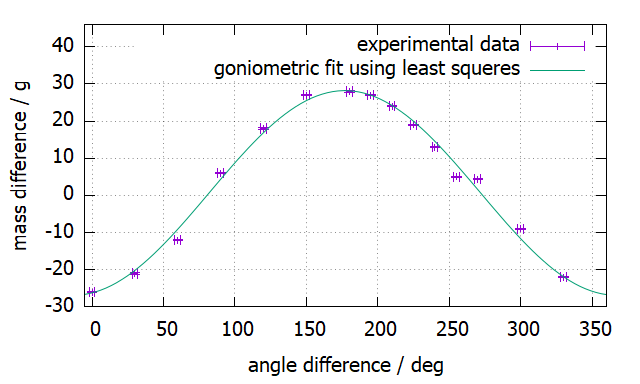
\includegraphics[width=0.8\textwidth]{Oleguv_graf.png}
  \caption{Dependence of magnetic force on angle difference}
  \label{obr:uhel}
\end{figure}

\begin{figure}[H]
  \centering
  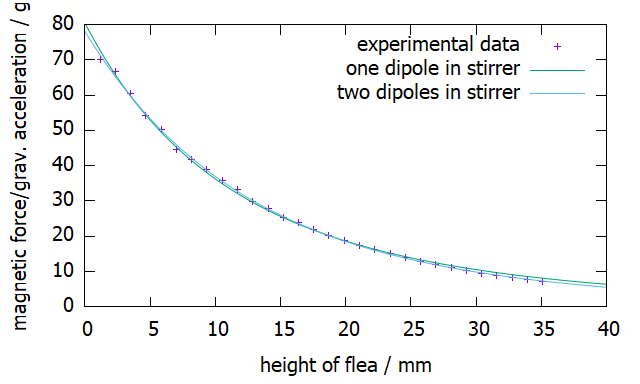
\includegraphics[width=0.8\textwidth]{blecha_sila-vyska.png}
  \caption{Dependence of magnetic force on flea height}
  \label{obr:vyska}
\end{figure}

\subsection{Magnetic forces - summary}
We created two different models of the effects of the magnets. Both approximate the flea as a magnetic dipole. The first one considers the stirrer magnets as a single point dipole; the second one as two dipoles. Both models correlate with our experiments. Due to the similarity of both models, we will be using the first one for further investigation to maintain simplicity. The equations involved are:
\begin{equation}
M_{mag} = \frac{K_{mag}}{h^3}\sin(\theta_f - \theta_{st})
\label{mmagshrnuti}
\end{equation}
and
\begin{equation}
F_{mag} = 3\frac{K_{mag}}{h^4}\cos(\theta_f - \theta_{st})
\label{fmagshrnuti}
\end{equation}

\section{Drag forces in viscous fluids}
Another important factor, which has an effect on the phenomenon, is the viscosity of the fluid, or more precisely,  the resistance due to the viscosity. Like in the case of magnetic forces, the effects of the resistance can be divided into two sub-effects: the drag on horizontal rotation and the drag on vertical movement. First, we investigated the relations between drag moment and vertical force drag. Glycerol was used as a viscous fluid; we measured its viscosity and compared it to reference values.

\subsection{Theoretical model of drag force and drag moment}
For low velocities, the drag on an object inside a viscous fluid can be described as
\begin{equation}
\vec{F}_{drag} = - k l \mu \vec{v}
\label{dragobecne}
\end{equation}
Where $k$ is the geometric factor, $l$ the characteristic length, $\mu$ the dynamic viscosity, and $\vec{v}$ the velocity of the object. The flea used is approximately cylindrical, therefore it will be modeled as a cylinder. Drag in the vertical direction can be calculated analogically:
\begin{equation}
F_{d\, ver} = - k_1 l_{f} \mu v_{ver}
\label{dragsv}
\end{equation}
The value of the constant $k_1$ is based on the study by T. Shiau (2014). $l_f$ is thus the height of the cylinder. The more complex part is determining the moment of drag; the method we used divides the cylinder into a series of infinitely thin width. It can thus be computed as an integral:
\begin{equation}
 M_{d} = \int_{-\frac{l_f}{2}}^{\frac{l_f}{2}} - l_f \times k_2 \mu v dl = \int_{-\frac{l_f}{2}}^{\frac{l_f}{2}} - k_2 l_f^2 \mu \omega_f dl = - \frac{k_2}{12}l_f^3 \mu \omega_f 
 \label{dragrot}
 \end{equation}
The value of the constant $k_2$, is based on the research by Baldwin et al. (2018); $\omega_f$ is the angular velocity of the flea. Like in the previous sections, all the constants can be substituted for a single one:
\begin{equation}
 C_{ver} = k_1 l_{f} \mu 
 \label{cverdef}
 \end{equation}
and
\begin{equation}
 C_{rot} = \frac{k_2}{12}l_f^3 \mu 
 \label{crotdef}
 \end{equation}
the equations are thus reduced to
\begin{equation}
 F_{d \, ver} = - C_{ver} \, v_{ver}
 \label{Fdragfinal}
 \end{equation}
and
\begin{equation}
 M_{d} = - C_{rot} \, \omega_f 
 \label{Mdragfinal}
 \end{equation}

\subsection{Glycerol parameters}
To be able to quantify the variables in the above relations, the viscosity value must be obtained. The reference value for  glycerol at 20\degree C is about $1.41 Pa \cdot s$ (Segur and Oberstar, 1951; Glycerine Producers Association, 1963). To validate this value, we used the falling-ball experiment, one of the classic rheological methods. \ref{obr:viskometr}. The method is based on the assumption, that a free-falling ball (of a negligible momentum) will free-fall at a constant velocity in the liquid, which means the drag force is equal to the weight. This gives the following equation:
\begin{equation}
 m_b g = 6 \pi r_b \mu v
 \label{stokes}
 \end{equation}
The viscosity can then be calculated using the falling speed; in our experiment, we used a 5 mm wide marble and captured its motion with a high-speed camera; the speed was determined from this data, and from the speed, the viscosity was calculated. The value obtained was about $1.38 Pa \cdot s$, which corresponds well to the reference value.

\begin{figure}[H]
  \centering
  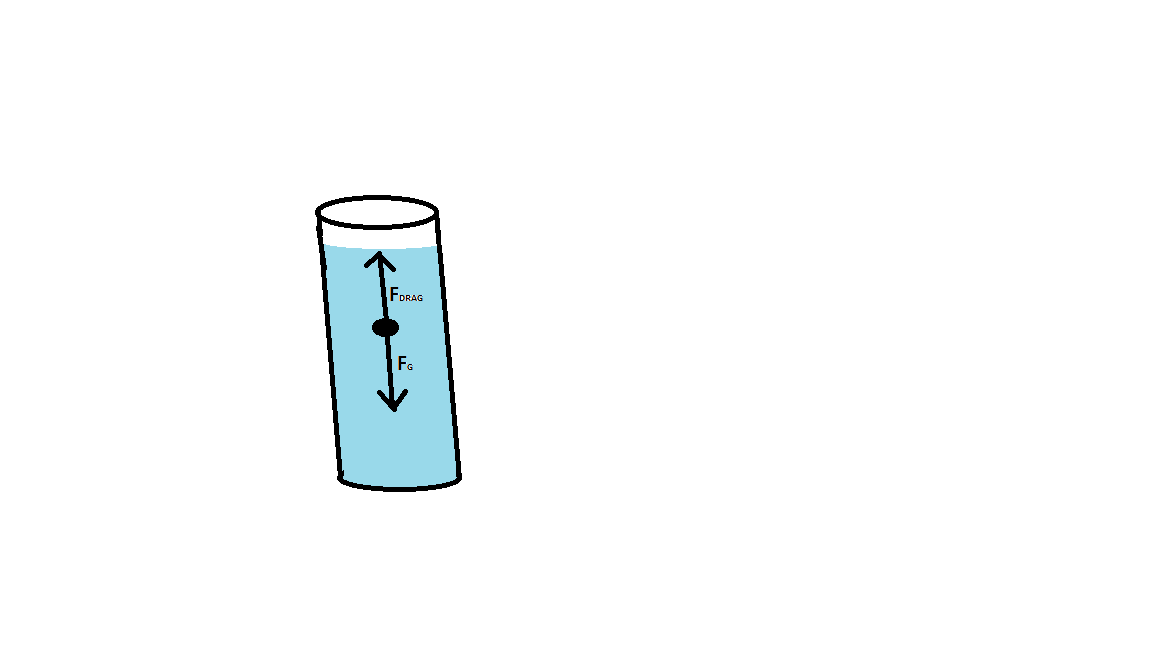
\includegraphics[width=0.5\textwidth]{viskozita_nakres.png}
  \caption{Viscosity measuring experiment scheme}
  \label{obr:viskometr}
\end{figure}

\section{Theoretical explanation and simulation}

\subsection{Qualitative analysis}
Our explanation of the phenomenon of levitation is based on the thought that the average magnetic force on the flea is directed upwards and has an equal magnitude to the gravitational force. The viscous fluid acts as a mediator, slowing down all movements in the phases where repulsion and attraction are imbalanced.
\subsection{Quantitative analysis}
The complicated movement of the flea consists, according to our models discussed above, of vertical and rotational components. For the horizontal rotation, the angular momentum theorem applies:
\begin{equation}
 \dot{L} = M_{mag} + M_d 
 \label{momenthybnosti}
\end{equation}
For vertical movement, the momentum theorem can be used:
\begin{equation}
 \dot{p}_{ver} = F_{G} + F_{b} + F_{mag} + F_{d \, ver} 
 \label{hybnost}
 \end{equation}
which can be extended into the following:
\begin{equation}
 I \ddot{\theta}_f = - C_{rot} \dot{\theta}_{f} + \frac {K_{mag}}{h^3} \sin(\theta_f - \omega_{st} t) 
 \label{rotace}
 \end{equation}
and
\begin{equation}
 m \ddot{h} = -m g + V \rho g - C_{ver} \dot{h} + 3 \frac{K_{mag}}{h^4} \cos(\theta_f - \omega_{st} t) 
 \label{svislypohyb}
 \end{equation}
which is a set of two simultaneous, non-linear, ordinary differential equations, describing the motion of the flea. Equivalent relations were found by already mentioned Baldwin, et al. (2018). The above equations are too complex to be solved analytically, therefore we decided to solve them numerically, using Euler's method. An iteration step size of  0.3 milliseconds was chosen to minimize errors; A re-run of the calculations with a step of 0.08 milliseconds had a negligible effect on the results, meaning the values are basically converged at the given step size. To be able to compute the results, a simulation was written in Processing (expanded Java). A model simulation can be found in the attachments.

\subsection{Determination of constants}
For the simulation to work, correct constant values have to be inputted; we measured the parameters. The flea diameter is $0.45 cm$ and the height $3.70 cm$, the volume of the flea is thus $2.35 cm^3$. The mass is $8.96 g$ The moment of inertia of the flea is evaluated according to the study by Zajíc (2010):
\begin{equation}
 I = \frac{1}{4} m \left( r^2 + \frac{l^2}{3} \right) 
 \label{momentsetrvacnosti}
 \end{equation}
leading to a value of $ 1.07 \cdot 10^{-6} \, kg.m^2 $. Furthermore, the composite constants defined earlier have to be calculated. $C_{ver}$ is equal to $0.69 \, kg.s^{-1}$, $C_{rot} = 4.99 \cdot 10^{-5} kg.m^2.s^{-1}$ and $K_{mag} = 8.04 \cdot 10^{-7} kg.m^5.s^{-2}$; The stirrer magnets are some distance underneath the bottom of the beaker, meaning this distance has to be taken into consideration when using this constant. The last constant needed is that of glycerol density; the reference value for 20\degree C is about $1261 kg.m^{-3}$ (GPA, 1963).

\section{Comparison of simulation and experiments}
Using the simulation, we constructed multiple predictions and compared them to experimental data.

\subsection{Flea trajectory}
The first comparison to experimental data focuses on the movement of the flea depending on time. To be able to use video tracking, we colored one side of the flea black; the result obtained from the video was the trajectory of the flea over time. When inputted into the simulation, a side-by-side visualization was created: the correlation between the predicted and measured behavior is well within measurement errors. An example can be found in the attachments.
\subsection{Levitation height}

\begin{figure}[H]
  \centering
  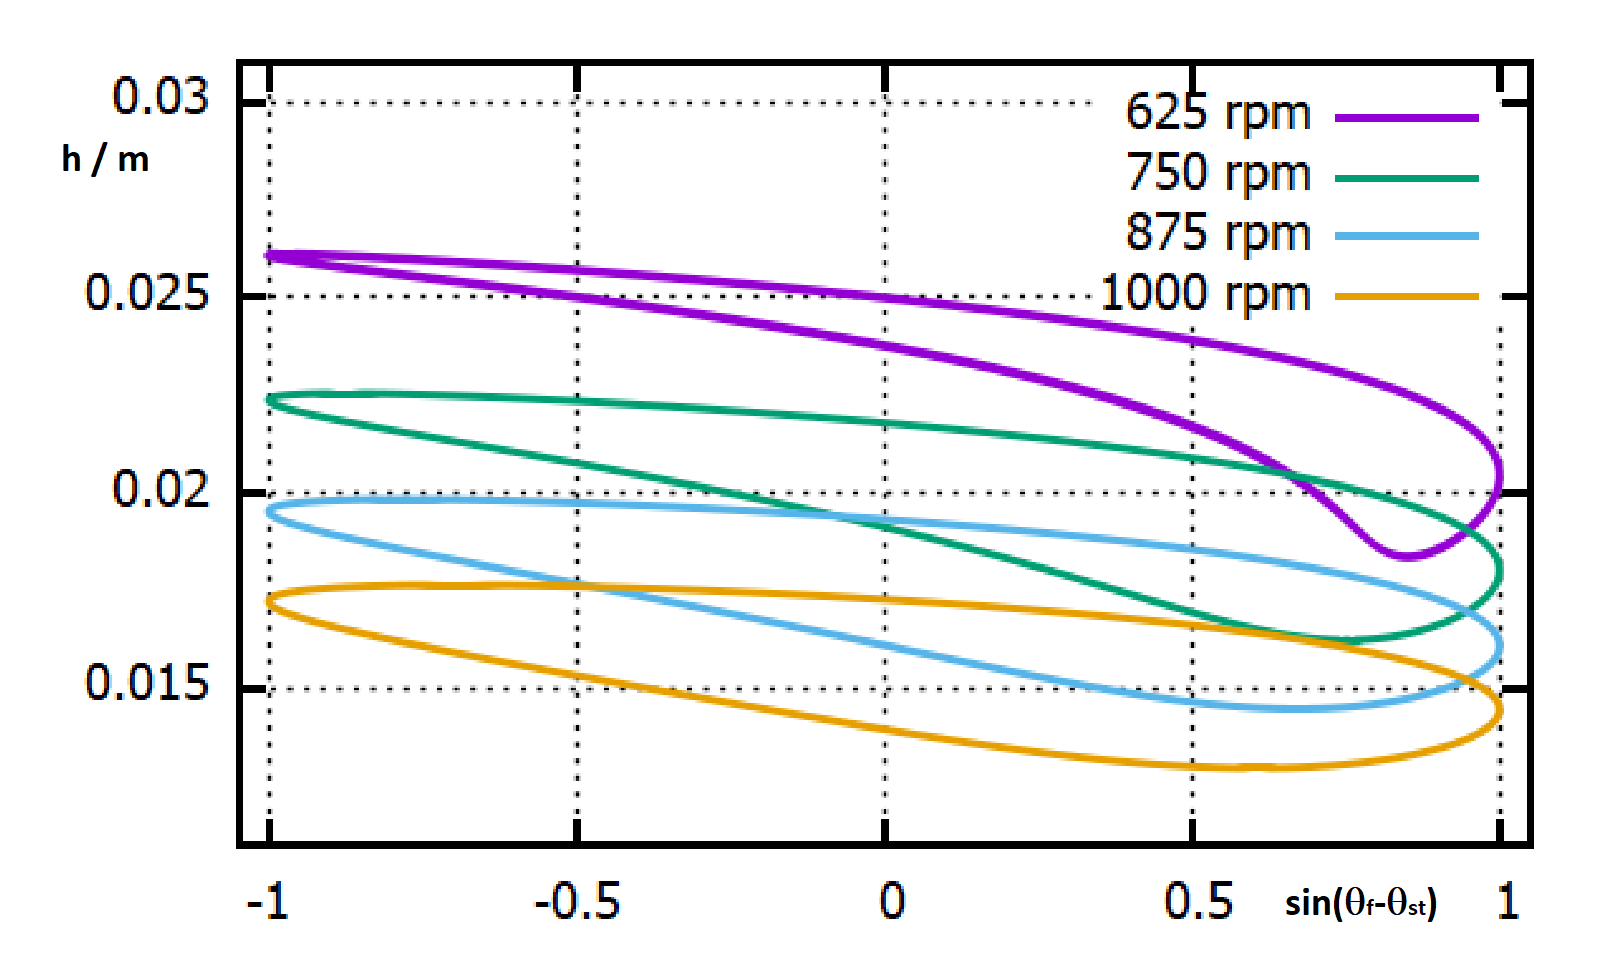
\includegraphics[width=0.8\textwidth]{atraktory.png}
  \caption{Dependency of flea height on angle distance for various angular velocities}
  \label{obr:atraktory}
\end{figure}

The next comparison aims to determine the height of levitation in dependence to stirrer magnet angular velocity. This is a more complex evaluation given that the height is not constant even at constant rotation velocities. Results of the simulation can be seen in graph \ref{obr:atraktory}.
The flea height in dependence to angle difference is characterized by these attractors. To verify the attractors, we tried several different starting positions of the flea. The output (as seen in the graph) is always a closed loop, meaning the system is deterministic, and not a chaotic system or deterministic chaos (for example, the Lorenz system). The system is thus not sensitive to small starting conditions' changes, which allows more room for further predictions. One may go so far to say, that the difference in angles and the rotation velocity is enough data to calculate the flea height, without knowing any of the system's past.\par It is also possible to notice, that the attractors, as rotation velocity increases, are at lower and lower heights, and also change in shape. Using a high-speed camera, we found that the difference between minimal and maximal flea height at 750 rpm is about $6 \, mm$, which is in accordance with the prediction (the corresponding attractor from image \ref{obr:atraktory}). We also tried measuring the height of the flea in the lowest point of the levitation. The method used is physical measuring with a ruler, which assumes that the flea oscillates so quickly, that the lowest point of the visible blur is the lowest point of oscillation. An overview of results can be seen in table \ref{tab:vysky}. It is notable, that the predicted values correlate to the measured ones, except for the value at 625 rpm. The inconsistency with 625 rpm can be explained by the sudden changes in movement (see graph \ref{obr:atraktory}), which could be unobservable using the human eye.

\begin{table}
\centering
\begin{tabular}{|c|c|c|c|}
\hline
rpm & height - theory / mm & height - experiment / mm & error / mm \\
\hline
625 & 18 - 26 & 23 & $\pm$1 \\
\hline
750 & 16 - 23 & 17 & $\pm$1 \\
\hline
875 & 14 - 20 & 14 & $\pm$1 \\
\hline
1000 & 13 - 18 & 12 & $\pm$1 \\
\hline
\end{tabular}
\caption{Comparison of predicted and measured values}
\label{tab:vysky}
\end{table}

\subsection{Angular velocity constraints}

Another area we investigated is the minimal angular velocity needed to sustain levitation. With a too low rotation velocity, the flea can not start hovering, as the magnets are not fast enough to create an inequality between attraction and repulsion large enough. The simulation predicted, that for 600 rpm and less, the flea would not levitate stably. Experimentally, we determined the minimum to be $600 \pm 30 \, ot/s$. The theoretical model thus checks out with the empirical. A recording of the flea in insufficient angular velocities can be found in the attachments.

\subsection{Sucrose solution}

Another component experiment, focused on using fluids of different viscosity, in particular, a sucrose solution. Using standard reference tables comparing concentration and viscosity (Subbiah and Morison, 2016), we obtained the solution's viscosity. The viscosity of a saturated solution was not enough to successfully reach a levitating state; both the experiment, and the simulations showed that the effect happening will instead be a stabilization of the flea's north and south poles above the stirrer's south and north poles, respectively, leading to attraction. To confirm this, we calculated that a fluid with the same density as glycerol, must have a viscosity of at least $0.7 Pa.s$ to support levitation.

\section{Additional observations}
This chapter aims to explore further observations, which are always either theoretical or experimental.

\subsection{Upper limit of viscosity}
For levitation to occur, the fluid has to have at least a minimal viscosity, determined above; we also investigated, if there exists a maximal viscosity. The simulation was re-ran for higher values. The general resulting trend was, that with higher viscosity, the flea levitates lower. At 5 times the glycerol viscosity, the flea was predicted to levitate lower than the beaker bottom, meaning a too high viscosity is not viable for the experiment. The qualitative explanation is based on the assumption that the magnetic forces are no longer strong enough to induce the characteristic movement of the flea.

\subsection{Changing flea size}
We tried substituting the flea for a smaller one; the observed levitation was only present at about 1000 rpm, at which the flea levitated at about a 1 cm height. As seen in image \ref{obr:atraktory}, higher rotation velocities lead to lower levitation, meaning the smaller flea can't levitate at more than about 1 cm height. 

\subsection{Approximation to $ \sin(x) + x $}
Again, Baldwin et al. (2018) managed to obtain similar equations describing the motion of the flea (\ref{rotace} and \ref{svislypohyb}). The study also claims, that the solution is a function for the angle:
\begin{equation}
 \theta_f = c_1 t + c_2\sin(c_3 \, t)
\label{sinx+x}
\end{equation}
  
\begin{figure}[H]
  \centering
  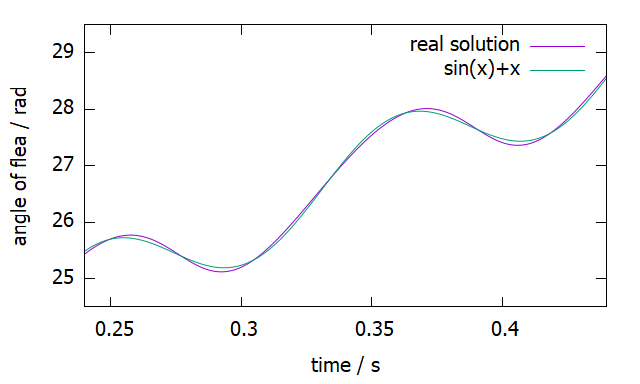
\includegraphics[width=0.8\textwidth]{rozdil_my_notingham.png}
  \caption{Comparison of $\sin(x)+x$ and numeric solution}
  \label{obr:sinx+x}
\end{figure}
  
where $c_1$, $c_2$ and $c_3$ are unknown constants. We compared this presumption with our numerical solution; the constants were determined by substituting a number of close points instead of the real solution, and applying the method of least squares. The results can be found in image \ref{obr:sinx+x}. It is visible that the function from equation \ref{sinx+x} correlates well to the numerical solution. Therefore, we tried re-calculating the simulation using this function instead of equation \ref{rotace}. Interestingly, only by changing the angle calculation, the predicted levitation height increased by about $20\%$, which would no longer correlate so well to the values obtained experimentally. We presume that this is due to a change in the ratio of attraction and repulsion times. It is remarkable, how such a small change is so prominent in the resultant simulation.

\subsection{Lissajous figures for this system}
For some certain angular velocities, interesting phase diagrams of flea angle and stirrer angle are formed; as an example, an angular velocity of $72.9624 \, rad.s^{-1}$ produces a phase diagram that can be seen in image \ref{lissajus}. The horizontal and the vertical axis, in this order, represent the cosine of stirrer magnets' angle and the cosine of the flea's. However, for different rotations, the white tracer will gradually cover the whole area.

\begin{figure}[H]
  \centering
  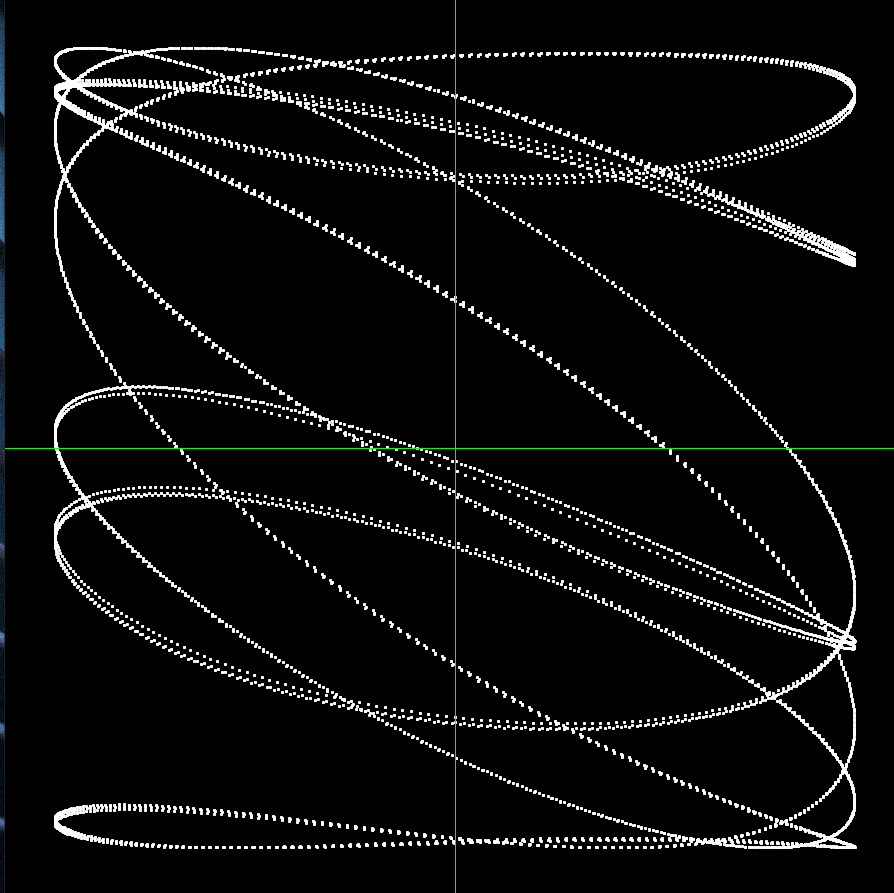
\includegraphics[width=0.5\textwidth]{faz.png}
  \caption{a phase diagram of rotation: $72.9624 \, rad.s^{-1}$}
  \label{lissajus}
\end{figure}

\section{Conclusion}
\subsection{Summary of achieved results}
In this research, we investigated the given phenomenon; we created two models to describe the behaviour of the system and proved both correlate well to experimental data. We explored how the viscous environment affects the flea of the stirrer, and compared our findings to experiments with glycerol. The resultant model consists of two non-linear differential equations, which we solved using Euler's method. A simulation was created on this basis and compared to various experimental data: flea rotation, which had a remarkable correlation (see attached videos); and flea height. Attractors were used to describe the flea height based on the angle difference. We managed to predict the minimal angular velocity needed and explain the role of viscosity in the phenomenon.

\subsection{Further research}
An area for further research could be improving the methods of measuring the flea levitation height; another area is to expand the calculations and simulations involved for different flea sizes; finally, an experiment giving some more insight into the flea's behaviour in differently viscous fluids would help in validating the predictions made in this area.


\section{Nomenclature} 
$\vec{B}$ - magnetic induction \newline
$\vec{B_{f}}$ - magnetic induction at the flea \newline
$c_i$ - unknown arbitrary constant \newline
$C_{rot}$ - drag moment constant $ = \frac{k_2}{12}l_f^3 \mu $ \newline
$C_{ver}$ - drag force constant $ = k_1 l_{f} \mu $ \newline
$f_b$ - buoyancy force \newline
$\vec{F_{drag}}$ - drag in a viscous fluid \newline
$F_{d \, ver}$ - drag against vertical motion \newline
$F_G$ - weight \newline
$F_{mag}$ - vertical force on the flea from the magnets \newline
$g$ - gravitational acceleration \newline 
$h$ - flea height \newline
$I$ - flea moment of inertia \newline
$k$ - geometric factor \newline
$k_1$ - geometric factor for vertical motion \newline
$k_2$ - geometric factor for cylinder rotation \newline
$K_{mag}$ - composite constant for describing magnetic fields $= \frac{\mu_{0}}{4 \pi}{|\vec{m_f}||\vec{m_{st}}|}$\newline
$l$ - characteristic length \newline
$l_{f}$ - length of the flea (cylinder height) \newline
$L$ - angular momentum of the flea \newline
$m_b$ - marble mass \newline
$M_d$ - drag moment on the flea \newline
$M_{mag}$ - magnetic field force moment \newline
$\vec{m_f}$ - magnetic dipole moment of the flea dipole \newline
$\vec{m_{st}}$ - magnetic dipole moment of the dipole in the stirrer (single dipole model) \newline
$p_{ver}$ - vertical motion momentum of the flea \newline
$r$ - cylinder radius \newline
$\vec{r}$ - vector of flea orientation \newline
$r_b$ - marble radius \newline
$\vec{v}$ - velocity \newline
$v_{ver}$ - vertical flea speed \newline
$V$ - flea volume \newline
$x$ - distance of stirrer magnets from the axis of rotation (two dipole model) \newline
$\theta_f$ - flea rotation angle \newline
$\theta_{st}$ - stirrer dipole rotation angle \newline
$\mu$ - dynamic viscosity \newline
$\mu_0$ - vacuum permeability \newline
$\rho$ - fluid density \newline
$\omega_f$ - flea angular velocity \newline

\begin{thebibliography}{[2]}

\bibitem {jednota} - International Young Physicists’ Tournament. (2019, July 14). IYPT 2020 Problems. Retrieved from \url{https://iypt.org/wp-content/uploads/2019/07/IYPT_2020_Problems.pdf} 

\bibitem {notingham} - Baldwin, K. A.; de Fouchier, J.-B.; Atkinson, P.; Hill, R. J. A.; Swift, M. R.; \& Fairhurst, J. D. (2018, May 24). Magnetic Levitation Stabilized by Streaming Fluid Flows. Retrieved from \url{https://arxiv.org/abs/1805.08608}

\bibitem {bodovy_dipol} - Department of surface and plasma science, Charles University. (2017). Magnetický dipól. Retrieved March 23, 2020, from \url{https://physics.mff.cuni.cz/kfpp/skripta/kurz_fyziky_pro_DS/display.php/elmag/3_4}

\bibitem {odpor} - Shiau, T. (2014). Drag on a Cylinder in a Viscoelastic Stokes Flow. Retrieved from \url{https://tspace.library.utoronto.ca/bitstream/1807/44064/3/Shiau_Terence_C_20143_MASc_thesis.pdf}

\bibitem {viskozita} - Segur, J. B.; Oberstar, H. E. (1 September 1951). Viscosity of Glycerol and Its Aqueous Solutions. Industrial \& Engineering Chemistry 43 (9): 2117–2120. doi:10.1021/ie50501a040

\bibitem {moment setrvacnosti} - Zajíc, J. (2010). Momenty setrvačnosti geometricky pravidelných homogenních těles. Retrieved from \url{http://mech.fd.cvut.cz/education/bachelor/18sat/download/zajic_momenty_setrvacnosti.pdf}

\bibitem {hustota} - Glycerine Producers Association. (1963). Physical properties of glycerol and its solutions. Retrieved from \url{http://www.aciscience.org/docs/physical_properties_of_glycerine_and_its_solutions.pdf} 

\bibitem {sladky cuc} - Subbiah, B., \& Morison, K. (2016, June). Viscosity relationship for concentrated sugars at 20\degree C. Retrieved from \url{https://www.researchgate.net/figure/scosity-relationship-for-concentrated-sugars-at-20-C-Curves-for-sucrose-glucose-and_fig1_306477730}

\end{thebibliography}
\end{document} 